\chapter{Heritage of ice reservoirs}

\cleanchapterquote{Before the artificial glacier, we struggled to get any barley. But now we can grow many
  crops, even potatoes, which need to be planted earlier in the spring, but sell for much more money.
}{Tashi Tundup}{(A 76 year old farmer in Ladakh)}

This chapter provides conclusions based on research findings from data collected on AIRs in Switzerland and India,
as well as discussion and recommendations for future research. This chapter will review the purpose of the
study, research questions, literature review, and findings of the study. It will then present conclusions,
discussion of the conclusions, and recommendations for practice and for further research.

\section{Summary}

Cryosphere fed irrigation networks are completely dependant on the timely availability of meltwater from
glaciers, snow and permafrost. With the accelerated decline of glaciers, these irrigation networks can no longer
deliver adequate water to sustain agricultural output and take advantage of the complete growing season. As a
consequence, some mountain villages have either been abandoned or lie on the brink of desertification
\citep{grossmanHimalayanGlaciersMelt2015}.

In the past few decades, AIR technologies have provided much needed relief to these
water-stressed communities. These strategies revolve around augmenting their glacial ice reservoirs with
man-made ones that provide supplementary irrigation during the spring. In the context of the observed present
and predicted global glacier shrinkage, the development of such water storage technologies is crucial to ensure
continued sustenance of cryosphere-fed irrigation networks.

\begin{figure}[htb]
	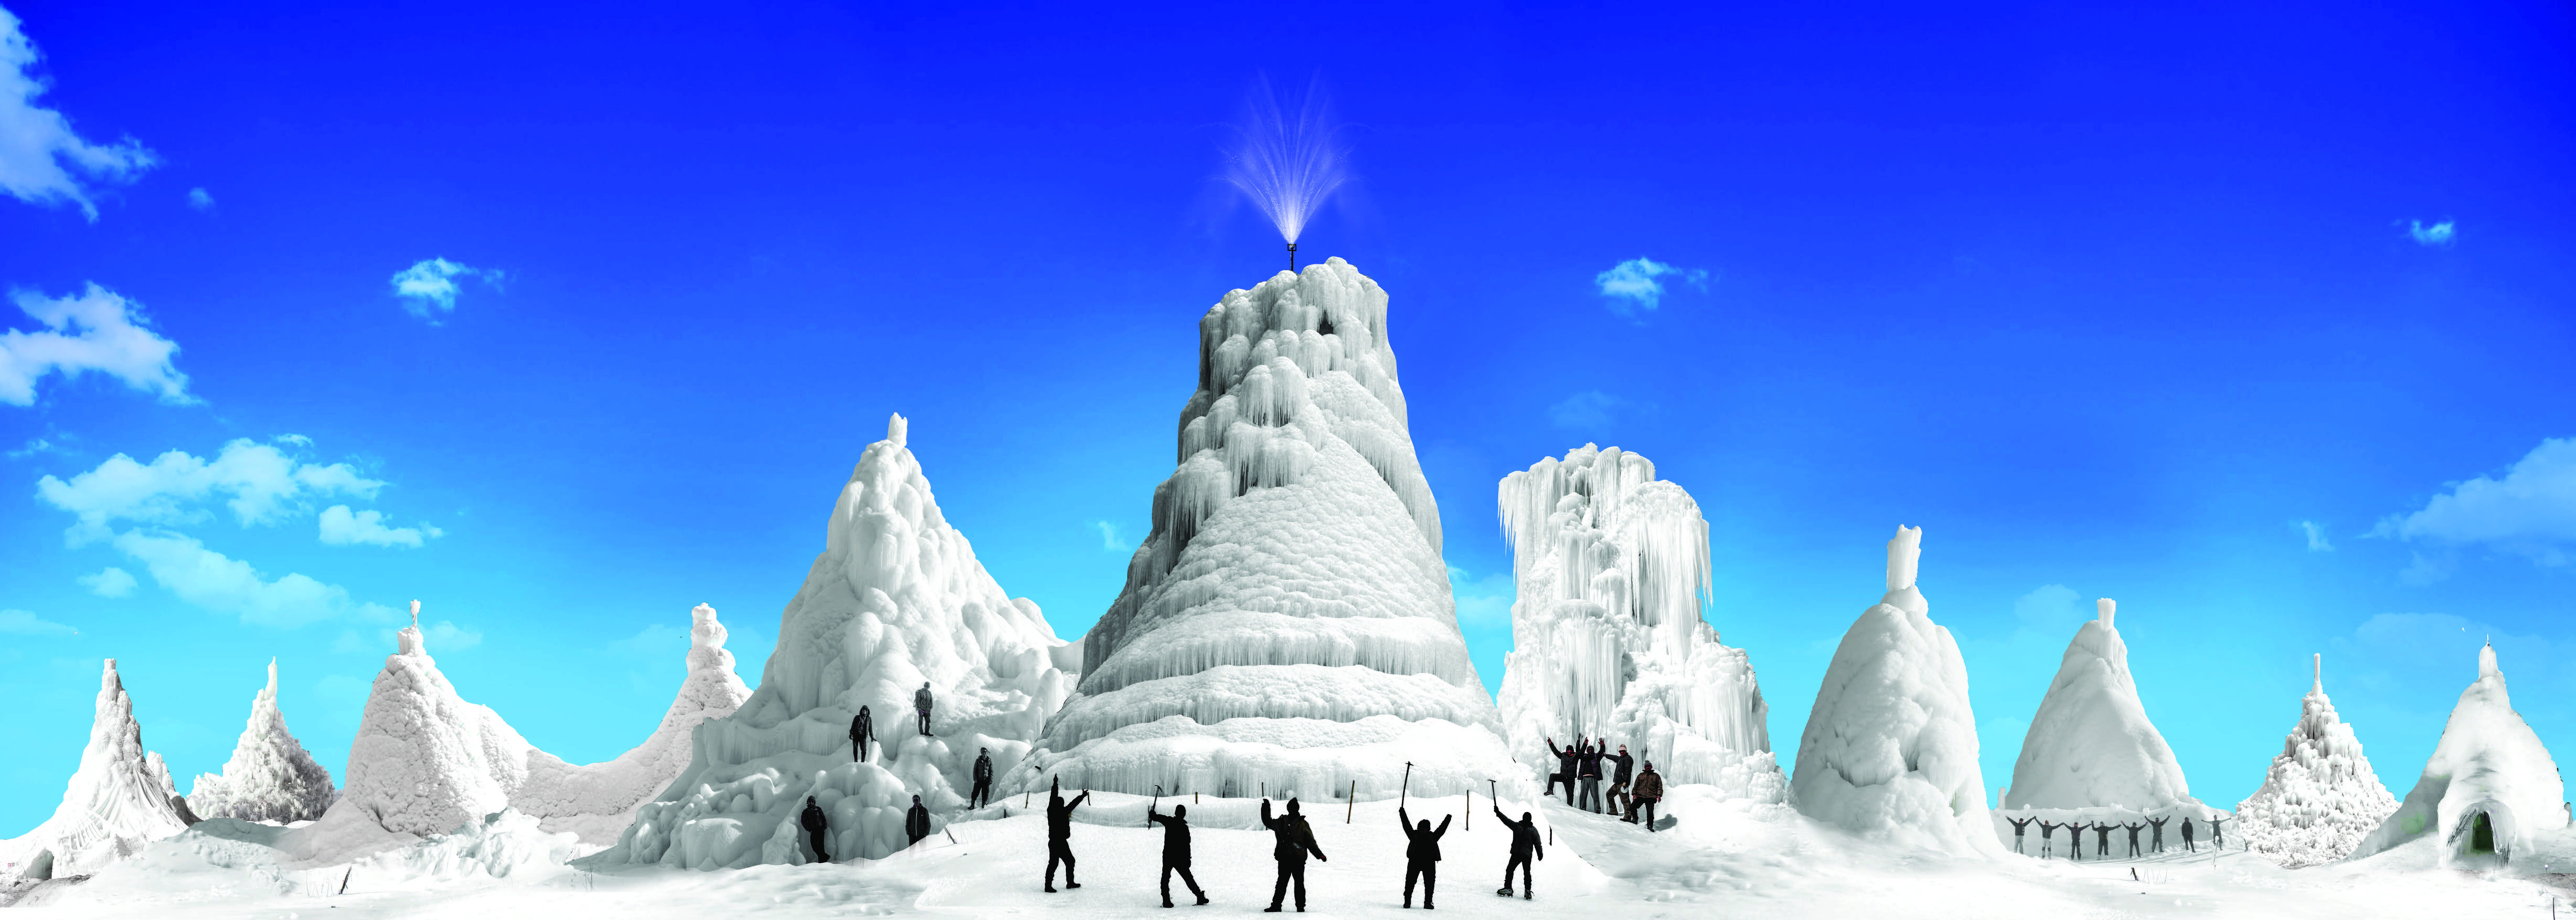
\includegraphics[width=\textwidth]{figs/AIRs_Ladakh}
	\caption{Compilation of AIRs built in different villages of Ladakh.}
	\label{fig:airs_ladakh}
\end{figure}

AIR observations and investigations date back to the mid-2000s \citep{tveitenGlacierGrowingLocal2007}. The vast
majority have been published in the 2010s, mostly using qualitative methods. However, quantifications of their
storage capacity differ widely amongst these publications \citep{baglaArtificialGlaciersHelp1998,
norphelSnowWaterHarvesting2015, nusserSociohydrologyArtificialGlaciers2019}. Because small-scale processes,
complex feedbacks and non-linearities govern their evolution, modelling the volume evolution of ice stupas is
only feasible if backed up with comprehensive input, calibration and validation datasets.

In response, we conducted measurement campaigns using drones, flowmeters and weather stations on almost a dozen
AIRs across two locations (India and Switzerland), over four winters (2019, 2020, 2021 and 2022) and using two
different construction methods (traditional and automated). Each dataset contained information on the
meteorological conditions, fountain characteristics and AIR volume evolution. 

The primary objective of this thesis was to improve our understanding about the response of AIRs to changes in
their construction location. The secondary objective was to propose automated constuction strategies that reduce
water losses and maintenance efforts.  

\section{Conclusions}

\begin{figure}[htb]
	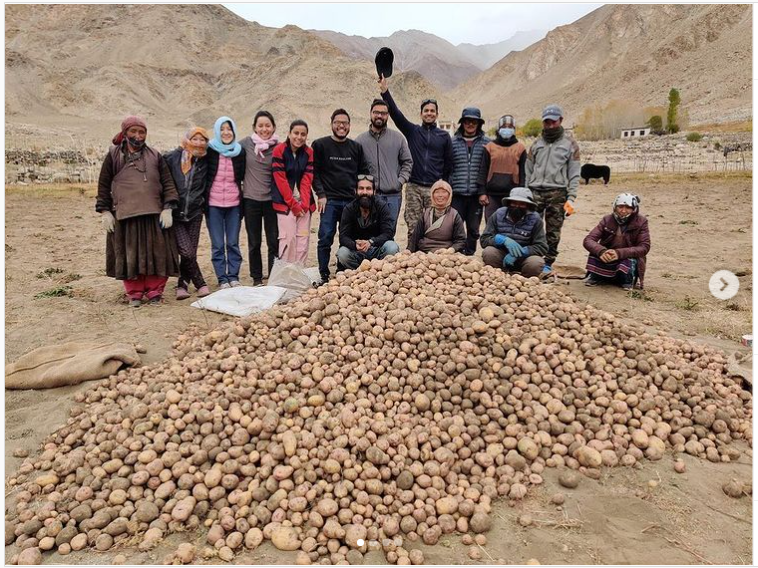
\includegraphics[width=\textwidth]{figs/Kullum_potatoes}
	\caption{One of the deserted villages in Ladakh where AIR meltwater supported a harvest of 1300 kgs of
  potatoes in October 2021. (P.C. Icestupa Project)}
	\label{fig:kullum_potatoes}
\end{figure}


In paper I, an AIR model was designed to resolve surface processes and used to compare their volume evolution
in Indian Himalayas and the Swiss Alps. In paper II, the evolution of AIRs using different fountain
scheduling strategies were compared. In paper III, the possibility of sustaining artificial ice reservoirs
perpetually was explored. The results of these papers can be summarised as follows:

\begin{enumerate} 

\item Volumes of ice stupas located in different regions may differ by an order of magnitude. The differences
  could be attributed to the accelerated sublimation process in colder and drier regions.

\item Water losses of ice stupas may be upto 80 \% due to excessive water input. However, water supply
  management through fountain scheduling strategies can produce icestupas of similar volumes while reducing upto
  one-tenth of their water supply.

\item Traditional construction systems demand significant maintenance efforts since they are prone to freezing
  events in the fountain pipeline. However, automated construction systems can prevent these events to make the
  construction process maintenance-free.

\item There exist locations with favourable weather conditions that can sustain artificial ice reservoirs
  perpetually.

\end{enumerate}

\section{Discussion}

\subsection{The state of ice stupa technology}

The thesis shows one strategy that can improve the water-use efficiency of AIRs. We chose this strategy because
it enables the use of the AIR model in a simple and effective manner. But all these construction strategies are
limited by the tools they use namely, the fountain and the pipeline. The fountain nozzle design is crucial for
increasing the ice volume obtained. However, no methodology currently exists to rank the several fountain
nozzles used for construction. An ideal pipeline configuration could make this technology cheaper and
maintenance free. However, optimization of the pipeline material and diameters is yet to be performed---despite
the time lost on pipeline freezing events and the potential cost reduction with cheaper pipeline materials and
sizes. Therefore, we strongly encourage the engineering community to get involved and push the limits of the
cost-effectiveness, size, and survival duration of artificial ice reservoirs. 

\subsection{Adaptation potential of glacierized catchments with AIRs}

Vanishing glaciers, natural hazards (like inundations, mudflows, and landslides), decreasing river discharge,
drying springs, next to shifts in precipitation patterns are apparent climate change impacts noticed by
glacierized catchments.

In the Peruvian Andes, both water scarcity (low-flow water risk) and glacial lake outburst floods (high flow
water risks) could have important impacts on local population, infrastructure and economic activities
\citep{motschmannIntegratedAssessmentsWater2020}. For example, the estimated loss in wheat output due to reduced
glacial runoff would be to the tune of 18 million USD in the low emission scenorio of Quillcay catchment of Peru
\citep{motschmannCurrentFutureWater2022}. Similarly, in the Stok catchment of Ladakh, glacial ice reserves have
shrunk by more than 18 \% in the past 16 years  leading to a decline in crop productivity
\citep{sohebSpatiotemporalQuantificationKey2022}. 

We believe, AIRs can already buffer against low flow water risks in certain catchments. For example, ice
terraces in nearby valleys have been measured with areas upto 19 \% of the Stok glacier (0.8 $km^2$). With further technology
development, AIRs can also be used to mitigate high flow water risks. The glacial lakes of the Andes and
Himalayas can be siphoned to form AIRs in scale that last perpetually. Such AIRs can compound over the years to
become another source of perennial water supply for the respective catchments.

\section{Future research direction}

\TODO{Expand}

Any future research can take advantage of the weather, fountain and drone datasets acquired in the two field
sites described in this thesis. Both AIR and COSISTUPA models are also freely provided through git repositories
for non-profit purposes (https://github.com/gayashiva, last access: August 1, 2022).

Insights from this research could contribute to efforts to better estimate the future potential of AIRs for
climate change adaptation and mitigation under multiple plausible future climatic, demographic, economic, and
land use scenarios. 

\subsection{Model development}

The COSISTUPA model developed in section \ref{sec:Cosistupa} should be used for future estimations for AIR volume. This model
needs to be extended so that it can account for future climate variability and produce accurate meltwater
predictions. Modelling the future is fundamentally different from simulating the past: In the past the model
serves as a tool for interpreting and best exploiting field measurements - and can be directly constrained by
these. Models for the future must understand climate variability to be able to yield realistic projections.
Almost all methodological steps in the modelling of future AIR runoff are subject to possible enhancements,
always bearing in mind that we will only know whether the effort led to an enhanced or even a worsened
performance, when we're old...

\subsection{Quantification and development of ice terraces}

Although this thesis focuses on ice stupas, their ice volumes pale in comparison with ice terraces
\citep{nusserSociohydrologyArtificialGlaciers2019}. This is because ice stupas are limited by their fountain's
spray radius. However, ice terraces have no such limitations. Their thickness is only limited by the water
supply rate or weather conditions and they can occupy any construction area provided. But despite this, ice
stupas are the preferred method of ice harvesting due to their longer survival duration and reduced construction
effort.

With a suitable redesign of the automation hardware, automated construction strategies can also be applied on
ice terraces. Such a construction strategy can potentially compound their size every consecutive winter with
minimal maintenance requirements. Therefore, future research direction should aim to answer the following
questions:

\begin{itemize}

  \item How can ice terrace construction systems be engineered to reduce their water losses and maintenance
    efforts?

\end{itemize}

The methodology developed in this thesis should also apply for such an analysis.

\subsection{Quantifying sustenance of glacierized catchments with AIRs}

Glaciers provide an important buffer for highly seasonal precipitation regimes
\citep{kaserContributionPotentialGlaciers2010}. Under the currently available climate change projections it is
expected that glacial mass loss will continue in future decades, and that several smaller glaciers will continue
to dissapear completely \citep{rabatelCurrentStateGlaciers2013}. 

In arid and semiarid regions, in particular, it is estimated that between 50 \% and 90 \% of freshwater
resources originate from mountain catchments \citep{messerliMountainsWorldVulnerable2004}. During drought
conditions in the tropical mountain regions, glacial meltwater is used by upto 3.92 million domestic users and
to irrigate 2096 $km^2$ of land \citep{buytaertGlacialMeltContent2017}.  

These trends stress the importance of increased water storage capacity for glacierized catchments as a pathway
for climate adaptation. Because of the challenges and cost related to traditional storage efforts, AIRs can be
a better tool to adapt against reduced glacial runoff. In order to quantify their adaptation potential, it
is necessary to understand the changing dynamics of AIR melting, but also map how their meltwater contributes to
current and future water use. While the spatiotemporal dynamics of AIR melt are increasingly well understood and
documented in this thesis, major uncertainty remains on how their meltwater contribution propagates through the
hydrological system and compares against the total discharge of mountain catchments. 

Future research needs to determine which catchments can benefit most from the supplementary water supply
provided by these ice harvesting technologies and flag off the urgent climate action required to increase their
water security.

% Finally, the scripts developed are also shared and could be adapted in various contexts to
% efficiently calculate ice surface processes over arbitrary complex and/or large geometries, including in
% non-mountain applications; a further benefit of the “Open Science” approach taken.

% \section{Final thoughts}

% Progressing glacier melt and the associated growing number of lakes rises the threat of glacier lake outburst
% floods (GLOFs); at the same time declining melt water supply changes the hydological regime, resulting in
% changing water availability especially during dry seasons. AIRs could become a crucial water resource management
% strategy to deal with both these high and low flow water hazards.

% With suitable technological development, GLOF risk can be mitigated through artificial glaciers.

% Successfully creating such an artificial glacier could provide unprecedented scientific insights in the
% processes governing glacial formation. More importantly, they could be used to harvest glacial lakes into ice
% reservoirs and pave the way for scalable climate adaptation strategies.

% \subsubsection{Educational tool}

% , climate change communication, scientific experiments

% \subsubsection{Sustainable tourism}

% Sculpture, religious monument, accomodation, ice climbing

% The model has been shown to perform excellently when calibrated with the AIR datasets.  It could be shown that
% the maximum volume of AIRs located in the IN and CH regions differ by an order of magnitude. These differences
% were caused by the stronger sublimation process due to the colder and drier weather conditions of the IN region. 

% AIR maintenance requirement was reduced and their fountain freezing events were prevented by developing an
% automated construction strategy. Fountain operation was made 8 times more efficient and effortless through the
% use of an automation system that scheduled discharge rates based on the recommendations of the AIR model. 

% For example, the catchment of Chicon, Peru has a current glacier coverage of more than 6 \%. In general, the
% runoff in Chicon is low, barely exceeding 1.2 $m^3/s$ even during the wet season. Runoff during the dry months
% is very low and goes down to only 0.2 $m^3/s$ \cite{motschmannIntegratedAssessmentsWater2020}. The glacier
% meltwater contribution is comparatively low but still has an important impact. The situation potentially worsens
% in the future, where the runoff in the high emission scenorio is constantly below 1 $m^3/s$ and goes down to 0.1
% $m^3/s$.

% Glaciers, seasonal snow, and permafrost buffer flow in water catchments between the dry and wet seasons. 
